% Options for packages loaded elsewhere
\PassOptionsToPackage{unicode}{hyperref}
\PassOptionsToPackage{hyphens}{url}
%
\documentclass[
]{article}
\usepackage{amsmath,amssymb}
\usepackage{iftex}
\ifPDFTeX
  \usepackage[T1]{fontenc}
  \usepackage[utf8]{inputenc}
  \usepackage{textcomp} % provide euro and other symbols
\else % if luatex or xetex
  \usepackage{unicode-math} % this also loads fontspec
  \defaultfontfeatures{Scale=MatchLowercase}
  \defaultfontfeatures[\rmfamily]{Ligatures=TeX,Scale=1}
\fi
\usepackage{lmodern}
\ifPDFTeX\else
  % xetex/luatex font selection
\fi
% Use upquote if available, for straight quotes in verbatim environments
\IfFileExists{upquote.sty}{\usepackage{upquote}}{}
\IfFileExists{microtype.sty}{% use microtype if available
  \usepackage[]{microtype}
  \UseMicrotypeSet[protrusion]{basicmath} % disable protrusion for tt fonts
}{}
\makeatletter
\@ifundefined{KOMAClassName}{% if non-KOMA class
  \IfFileExists{parskip.sty}{%
    \usepackage{parskip}
  }{% else
    \setlength{\parindent}{0pt}
    \setlength{\parskip}{6pt plus 2pt minus 1pt}}
}{% if KOMA class
  \KOMAoptions{parskip=half}}
\makeatother
\usepackage{xcolor}
\usepackage[margin=1in]{geometry}
\usepackage{color}
\usepackage{fancyvrb}
\newcommand{\VerbBar}{|}
\newcommand{\VERB}{\Verb[commandchars=\\\{\}]}
\DefineVerbatimEnvironment{Highlighting}{Verbatim}{commandchars=\\\{\}}
% Add ',fontsize=\small' for more characters per line
\usepackage{framed}
\definecolor{shadecolor}{RGB}{248,248,248}
\newenvironment{Shaded}{\begin{snugshade}}{\end{snugshade}}
\newcommand{\AlertTok}[1]{\textcolor[rgb]{0.94,0.16,0.16}{#1}}
\newcommand{\AnnotationTok}[1]{\textcolor[rgb]{0.56,0.35,0.01}{\textbf{\textit{#1}}}}
\newcommand{\AttributeTok}[1]{\textcolor[rgb]{0.13,0.29,0.53}{#1}}
\newcommand{\BaseNTok}[1]{\textcolor[rgb]{0.00,0.00,0.81}{#1}}
\newcommand{\BuiltInTok}[1]{#1}
\newcommand{\CharTok}[1]{\textcolor[rgb]{0.31,0.60,0.02}{#1}}
\newcommand{\CommentTok}[1]{\textcolor[rgb]{0.56,0.35,0.01}{\textit{#1}}}
\newcommand{\CommentVarTok}[1]{\textcolor[rgb]{0.56,0.35,0.01}{\textbf{\textit{#1}}}}
\newcommand{\ConstantTok}[1]{\textcolor[rgb]{0.56,0.35,0.01}{#1}}
\newcommand{\ControlFlowTok}[1]{\textcolor[rgb]{0.13,0.29,0.53}{\textbf{#1}}}
\newcommand{\DataTypeTok}[1]{\textcolor[rgb]{0.13,0.29,0.53}{#1}}
\newcommand{\DecValTok}[1]{\textcolor[rgb]{0.00,0.00,0.81}{#1}}
\newcommand{\DocumentationTok}[1]{\textcolor[rgb]{0.56,0.35,0.01}{\textbf{\textit{#1}}}}
\newcommand{\ErrorTok}[1]{\textcolor[rgb]{0.64,0.00,0.00}{\textbf{#1}}}
\newcommand{\ExtensionTok}[1]{#1}
\newcommand{\FloatTok}[1]{\textcolor[rgb]{0.00,0.00,0.81}{#1}}
\newcommand{\FunctionTok}[1]{\textcolor[rgb]{0.13,0.29,0.53}{\textbf{#1}}}
\newcommand{\ImportTok}[1]{#1}
\newcommand{\InformationTok}[1]{\textcolor[rgb]{0.56,0.35,0.01}{\textbf{\textit{#1}}}}
\newcommand{\KeywordTok}[1]{\textcolor[rgb]{0.13,0.29,0.53}{\textbf{#1}}}
\newcommand{\NormalTok}[1]{#1}
\newcommand{\OperatorTok}[1]{\textcolor[rgb]{0.81,0.36,0.00}{\textbf{#1}}}
\newcommand{\OtherTok}[1]{\textcolor[rgb]{0.56,0.35,0.01}{#1}}
\newcommand{\PreprocessorTok}[1]{\textcolor[rgb]{0.56,0.35,0.01}{\textit{#1}}}
\newcommand{\RegionMarkerTok}[1]{#1}
\newcommand{\SpecialCharTok}[1]{\textcolor[rgb]{0.81,0.36,0.00}{\textbf{#1}}}
\newcommand{\SpecialStringTok}[1]{\textcolor[rgb]{0.31,0.60,0.02}{#1}}
\newcommand{\StringTok}[1]{\textcolor[rgb]{0.31,0.60,0.02}{#1}}
\newcommand{\VariableTok}[1]{\textcolor[rgb]{0.00,0.00,0.00}{#1}}
\newcommand{\VerbatimStringTok}[1]{\textcolor[rgb]{0.31,0.60,0.02}{#1}}
\newcommand{\WarningTok}[1]{\textcolor[rgb]{0.56,0.35,0.01}{\textbf{\textit{#1}}}}
\usepackage{graphicx}
\makeatletter
\def\maxwidth{\ifdim\Gin@nat@width>\linewidth\linewidth\else\Gin@nat@width\fi}
\def\maxheight{\ifdim\Gin@nat@height>\textheight\textheight\else\Gin@nat@height\fi}
\makeatother
% Scale images if necessary, so that they will not overflow the page
% margins by default, and it is still possible to overwrite the defaults
% using explicit options in \includegraphics[width, height, ...]{}
\setkeys{Gin}{width=\maxwidth,height=\maxheight,keepaspectratio}
% Set default figure placement to htbp
\makeatletter
\def\fps@figure{htbp}
\makeatother
\setlength{\emergencystretch}{3em} % prevent overfull lines
\providecommand{\tightlist}{%
  \setlength{\itemsep}{0pt}\setlength{\parskip}{0pt}}
\setcounter{secnumdepth}{-\maxdimen} % remove section numbering
\ifLuaTeX
  \usepackage{selnolig}  % disable illegal ligatures
\fi
\usepackage{bookmark}
\IfFileExists{xurl.sty}{\usepackage{xurl}}{} % add URL line breaks if available
\urlstyle{same}
\hypersetup{
  pdftitle={Project\_1\_456},
  pdfauthor={Anthony Yasan, Preston O'Connor, Khoa Dao, Matthew Jacob, Nick Wierzbowski},
  hidelinks,
  pdfcreator={LaTeX via pandoc}}

\title{Project\_1\_456}
\author{Anthony Yasan, Preston O'Connor, Khoa Dao, Matthew Jacob, Nick
Wierzbowski}
\date{2025-02-26}

\begin{document}
\maketitle

We are modeling the linear regression of the Dependent Income,
Independent Age in our model

\section{Introduction}\label{introduction}

Our model is a simple linear regression representing the relationship
between the feature age and result household income in the United
States. For our data we chose to use an extract from IPUMS USA, a
database that provides access to census and survey data for research
purposes. For our variable selection, we chose individual age and
household income; although this selection may seem counter intuitive, we
thought it pertinent to avoid bias in contributions to household income
stemming from homemaking and dependents. In this data extract household
income includes every member's individual annual incomes added up at
time of the census, referring to either their current annual salary or
their earnings in the last 12 months. Age is simply their current age at
the time of the census, and to avoid issues we filtered our sample to
include only 18-65 year old individuals to capture working age incomes.
The significance of this relation is its connection to the causes of
income inequality in the United States. If income is closely tied to
age, this suggests that income inequality is dependent on age bracket
and correlated years of experience, providing evidence of a degree of
social mobility across class. If this were the case, it may dissipate
political will from the lower classes to demand redistributive policies,
according to the POUM (prospect of upward mobility) hypothesis advanced
by Benanbou and Ok. However, a simple linear regression is definitely
not the best tool we could use to analyze this relation, as explained by
Solon that due to poor data selection (not analyzing the same households
or individuals across many years), and his more advanced model produces
a higher correlation between income and intergenerational income (which
is a slightly different question that ours). The packages used were
ipumsr, dplyr, ggplot2 and caTools. Ipumsr provides an easy interface to
access IPUMS data in r and even create extracts. Dplyr provides many
useful data manipulation tools, which include such functions as mutate
and filter. Ggplot2 provides the tools to easily create graphics
representing data and statistics. CaTools provides utility functions for
moving window statistics. Our results primarily indicate the weakness of
the model in relating our two variables, showing close to no correlation
between different individuals ages and their incomes. Again, considering
the more ideal elements of a similar analysis described by Solon this is
not a terribly surprising outcome.

\subsection{Installing the R-packages}\label{installing-the-r-packages}

\section{Data description}\label{data-description}

The dataset is sourced from IPUMS USA, which provides microdata
extracted from the U.S. Census and American Community Survey (ACS). It
contains demographic and economic data at both household and individual
levels.

The dataset consists of 3,405,809 rows and 15 columns.

However, for model implementation we randomly selected a seed of 200,000
rows to utilize for efficiency and for the modeling portion of our data.

Each observation represents a household.

Here are the key variables included in the dataset:\\
- YEAR: Census year (e.g., 2023).\\
- SAMPLE: IPUMS sample identifier.\\
- SERIAL: Unique household serial number.\\
- CBSERIAL: Original Census Bureau household serial number.\\
- HHWT: Household weight for proper representation.\\
- CLUSTER: Household cluster for variance estimation.\\
- STRATA: Household strata for variance estimation.\\
- GQ: Group quarters status (e.g., household, institution).\\
- HHINCOME: Total household income for all members over 15 years old. -
PERNUM: Person number within the household.\\
- PERWT: Person weight for population estimates.\\
- SEX: Gender classification (Male/Female).\\
- AGE: Individual's age in years.\\
- RACE: General race classification.\\
- RACED: Detailed race classification.

\subsection{Information about the Data
set}\label{information-about-the-data-set}

\begin{Shaded}
\begin{Highlighting}[]
\NormalTok{ddi }\OtherTok{\textless{}{-}} \FunctionTok{read\_ipums\_ddi}\NormalTok{(}\StringTok{"usa\_00001.xml"}\NormalTok{)}
\NormalTok{data }\OtherTok{\textless{}{-}} \FunctionTok{read\_ipums\_micro}\NormalTok{(ddi)}
\end{Highlighting}
\end{Shaded}

\begin{verbatim}
## Use of data from IPUMS USA is subject to conditions including that users should cite the data appropriately. Use command `ipums_conditions()` for more details.
\end{verbatim}

\begin{Shaded}
\begin{Highlighting}[]
\FunctionTok{dim}\NormalTok{(data)}
\end{Highlighting}
\end{Shaded}

\begin{verbatim}
## [1] 3405809      15
\end{verbatim}

\begin{Shaded}
\begin{Highlighting}[]
\FunctionTok{summary}\NormalTok{(data)}
\end{Highlighting}
\end{Shaded}

\begin{verbatim}
##       YEAR          SAMPLE           SERIAL           CBSERIAL        
##  Min.   :2023   Min.   :202301   Min.   :      1   Min.   :2.023e+12  
##  1st Qu.:2023   1st Qu.:202301   1st Qu.: 372386   1st Qu.:2.023e+12  
##  Median :2023   Median :202301   Median : 756830   Median :2.023e+12  
##  Mean   :2023   Mean   :202301   Mean   : 758992   Mean   :2.023e+12  
##  3rd Qu.:2023   3rd Qu.:202301   3rd Qu.:1147002   3rd Qu.:2.023e+12  
##  Max.   :2023   Max.   :202301   Max.   :1519010   Max.   :2.023e+12  
##       HHWT            CLUSTER              STRATA              GQ       
##  Min.   :   1.00   Min.   :2.023e+12   Min.   :  10001   Min.   :1.000  
##  1st Qu.:  48.00   1st Qu.:2.023e+12   1st Qu.: 100005   1st Qu.:1.000  
##  Median :  71.00   Median :2.023e+12   Median : 231248   Median :1.000  
##  Mean   :  97.24   Mean   :2.023e+12   Mean   : 488810   Mean   :1.134  
##  3rd Qu.: 115.00   3rd Qu.:2.023e+12   3rd Qu.: 480148   3rd Qu.:1.000  
##  Max.   :2225.00   Max.   :2.023e+12   Max.   :8100351   Max.   :5.000  
##     HHINCOME           PERNUM           PERWT              SEX       
##  Min.   : -16800   Min.   : 1.000   Min.   :   1.00   Min.   :1.000  
##  1st Qu.:  54000   1st Qu.: 1.000   1st Qu.:  47.00   1st Qu.:1.000  
##  Median : 100100   Median : 2.000   Median :  72.00   Median :2.000  
##  Mean   : 638692   Mean   : 2.058   Mean   :  98.34   Mean   :1.509  
##  3rd Qu.: 176400   3rd Qu.: 3.000   3rd Qu.: 117.00   3rd Qu.:2.000  
##  Max.   :9999999   Max.   :20.000   Max.   :2225.00   Max.   :2.000  
##       AGE             RACE           RACED      
##  Min.   : 0.00   Min.   :1.000   Min.   :100.0  
##  1st Qu.:22.00   1st Qu.:1.000   1st Qu.:100.0  
##  Median :44.00   Median :1.000   Median :100.0  
##  Mean   :43.11   Mean   :2.535   Mean   :257.9  
##  3rd Qu.:63.00   3rd Qu.:2.000   3rd Qu.:200.0  
##  Max.   :96.00   Max.   :9.000   Max.   :990.0
\end{verbatim}

\subsection{Table of Data}\label{table-of-data}

\begin{Shaded}
\begin{Highlighting}[]
\CommentTok{\#View(data)}
\CommentTok{\#The Code struggles to run the data set with 2 million points is two extensive to run, So select a random sample of 200,000 points}
\FunctionTok{set.seed}\NormalTok{(}\DecValTok{11}\NormalTok{)}

\NormalTok{s }\OtherTok{\textless{}{-}} \FunctionTok{sample}\NormalTok{(}\DecValTok{1}\SpecialCharTok{:}\FunctionTok{nrow}\NormalTok{(data), }\AttributeTok{size =} \DecValTok{200000}\NormalTok{)}
\NormalTok{data }\OtherTok{\textless{}{-}}\NormalTok{ data[s, ]}
\FunctionTok{dim}\NormalTok{(data)}
\end{Highlighting}
\end{Shaded}

\begin{verbatim}
## [1] 200000     15
\end{verbatim}

\subsection{Data Cleaning and Outlier
Removal}\label{data-cleaning-and-outlier-removal}

\begin{Shaded}
\begin{Highlighting}[]
\CommentTok{\# select the age and the Total Household income as the main columns of interest, then filter based of 18 \textless{}= age \textless{}= 65 (Thats the only age bracket that is currently working and has other factors effecting income). Also, there is a negative value in household income which doesn\textquotesingle{}t make sense at all, so we filter it out. }

\CommentTok{\# ask if the filter crashes out after a certain amount on the computer and if we need to shrink the train size}
\NormalTok{data }\OtherTok{\textless{}{-}}\NormalTok{ data }\SpecialCharTok{\%\textgreater{}\%}
  \FunctionTok{select}\NormalTok{(AGE, HHINCOME) }\SpecialCharTok{\%\textgreater{}\%}
  \FunctionTok{mutate}\NormalTok{(}\AttributeTok{HHINCOME =} \FunctionTok{as.numeric}\NormalTok{(HHINCOME), }\AttributeTok{AGE =} \FunctionTok{as.numeric}\NormalTok{(AGE)) }\SpecialCharTok{\%\textgreater{}\%}
  \FunctionTok{filter}\NormalTok{(}\SpecialCharTok{!}\FunctionTok{is.na}\NormalTok{(HHINCOME), }\SpecialCharTok{!}\FunctionTok{is.na}\NormalTok{(AGE)) }\SpecialCharTok{\%\textgreater{}\%}
  \FunctionTok{filter}\NormalTok{(}\FunctionTok{between}\NormalTok{(AGE, }\DecValTok{18}\NormalTok{, }\DecValTok{65}\NormalTok{)) }\SpecialCharTok{\%\textgreater{}\%}
  \FunctionTok{filter}\NormalTok{(HHINCOME }\SpecialCharTok{\textgreater{}} \DecValTok{0}\NormalTok{)}

\FunctionTok{dim}\NormalTok{(data)  }\CommentTok{\#if you want to view the two filtered columns}
\end{Highlighting}
\end{Shaded}

\begin{verbatim}
## [1] 117981      2
\end{verbatim}

\begin{Shaded}
\begin{Highlighting}[]
\NormalTok{IQR\_of\_AGE }\OtherTok{\textless{}{-}} \FunctionTok{IQR}\NormalTok{(data}\SpecialCharTok{$}\NormalTok{AGE, }\AttributeTok{na.rm =} \ConstantTok{TRUE}\NormalTok{)}
\NormalTok{IQR\_of\_HHINCOME }\OtherTok{\textless{}{-}} \FunctionTok{IQR}\NormalTok{(data}\SpecialCharTok{$}\NormalTok{HHINCOME, }\AttributeTok{na.rm =} \ConstantTok{TRUE}\NormalTok{)}


\NormalTok{AGE\_lower }\OtherTok{\textless{}{-}} \FunctionTok{quantile}\NormalTok{(data}\SpecialCharTok{$}\NormalTok{AGE, }\FloatTok{0.25}\NormalTok{, }\AttributeTok{na.rm =} \ConstantTok{TRUE}\NormalTok{) }\SpecialCharTok{{-}} \FloatTok{1.5} \SpecialCharTok{*}\NormalTok{ IQR\_of\_AGE}
\NormalTok{AGE\_upper }\OtherTok{\textless{}{-}} \FunctionTok{quantile}\NormalTok{(data}\SpecialCharTok{$}\NormalTok{AGE, }\FloatTok{0.75}\NormalTok{, }\AttributeTok{na.rm =} \ConstantTok{TRUE}\NormalTok{) }\SpecialCharTok{+} \FloatTok{1.5} \SpecialCharTok{*}\NormalTok{ IQR\_of\_AGE}

\NormalTok{HHINCOME\_lower }\OtherTok{\textless{}{-}} \FunctionTok{quantile}\NormalTok{(data}\SpecialCharTok{$}\NormalTok{HHINCOME, }\FloatTok{0.25}\NormalTok{, }\AttributeTok{na.rm =} \ConstantTok{TRUE}\NormalTok{) }\SpecialCharTok{{-}} \FloatTok{1.5} \SpecialCharTok{*}\NormalTok{ IQR\_of\_HHINCOME}
\NormalTok{HHINCOME\_upper }\OtherTok{\textless{}{-}} \FunctionTok{quantile}\NormalTok{(data}\SpecialCharTok{$}\NormalTok{HHINCOME, }\FloatTok{0.75}\NormalTok{, }\AttributeTok{na.rm =} \ConstantTok{TRUE}\NormalTok{) }\SpecialCharTok{+} \FloatTok{1.5} \SpecialCharTok{*}\NormalTok{ IQR\_of\_HHINCOME}

\CommentTok{\#continue to filter any of the outliers}
\NormalTok{filtered\_data }\OtherTok{\textless{}{-}}\NormalTok{ data }\SpecialCharTok{\%\textgreater{}\%}
  \FunctionTok{filter}\NormalTok{(AGE }\SpecialCharTok{\textgreater{}=}\NormalTok{ AGE\_lower }\SpecialCharTok{\&}\NormalTok{ AGE }\SpecialCharTok{\textless{}=}\NormalTok{ AGE\_upper)}\SpecialCharTok{\%\textgreater{}\%}
    \FunctionTok{filter}\NormalTok{(HHINCOME }\SpecialCharTok{\textgreater{}=}\NormalTok{ HHINCOME\_lower }\SpecialCharTok{\&}\NormalTok{ HHINCOME }\SpecialCharTok{\textless{}=}\NormalTok{ HHINCOME\_upper)}

\CommentTok{\# we check and see the data sets we have filtered out of here}
\FunctionTok{dim}\NormalTok{(filtered\_data) }
\end{Highlighting}
\end{Shaded}

\begin{verbatim}
## [1] 105383      2
\end{verbatim}

\subsection{Original Histogram}\label{original-histogram}

\subsubsection{Age}\label{age}

We can see in the histogram for Age that there is a relatively normal
distribution with no extreme skew or any outliers present at all.

\begin{Shaded}
\begin{Highlighting}[]
\FunctionTok{ggplot}\NormalTok{(data, }\FunctionTok{aes}\NormalTok{(}\AttributeTok{x =}\NormalTok{ AGE)) }\SpecialCharTok{+}
  \FunctionTok{geom\_histogram}\NormalTok{(}\AttributeTok{binwidth =} \DecValTok{5}\NormalTok{, }\AttributeTok{fill =} \StringTok{"blue"}\NormalTok{, }\AttributeTok{color =} \StringTok{"black"}\NormalTok{, }\AttributeTok{alpha =} \FloatTok{0.7}\NormalTok{) }\SpecialCharTok{+}
  \FunctionTok{labs}\NormalTok{(}\AttributeTok{title =} \StringTok{"Distribution of Age"}\NormalTok{, }\AttributeTok{x =} \StringTok{"Age"}\NormalTok{, }\AttributeTok{y =} \StringTok{"Frequency"}\NormalTok{) }\SpecialCharTok{+}
  \FunctionTok{theme\_minimal}\NormalTok{()}
\end{Highlighting}
\end{Shaded}

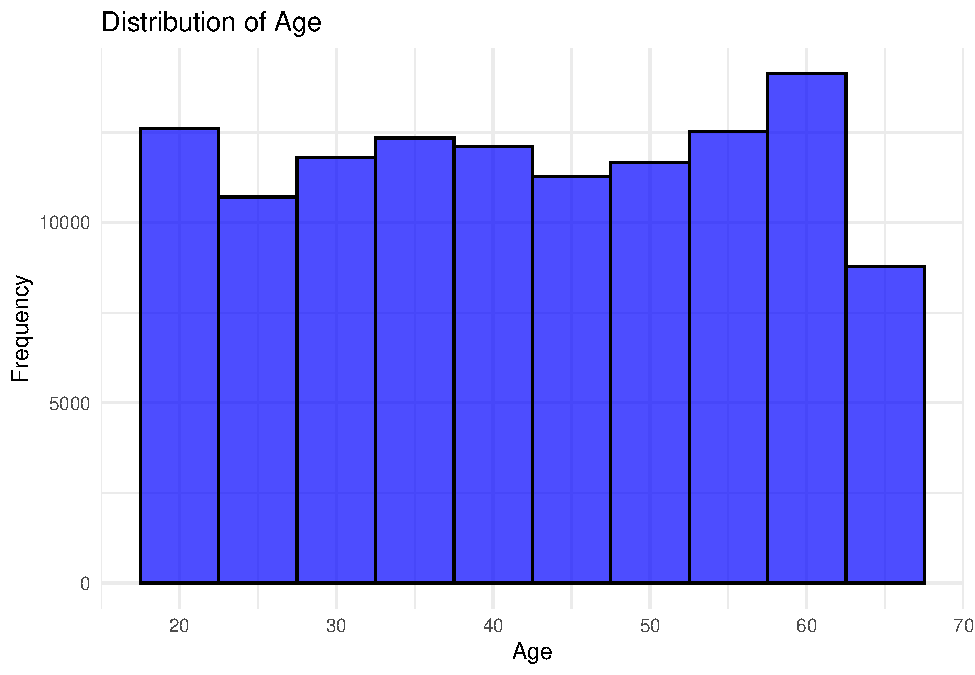
\includegraphics{Project_1_456_files/figure-latex/unnamed-chunk-5-1.pdf}

\subsubsection{Household Income}\label{household-income}

We can see here that pre-filtering our data has a very large right skew
and an extremely large outlier present in the data set.This is due to
the fact that most individuals earn a relatively modest and moderate
incomes.

It's likely this data set interviewed a lot of households who come from
this category.

\begin{Shaded}
\begin{Highlighting}[]
\FunctionTok{ggplot}\NormalTok{(data, }\FunctionTok{aes}\NormalTok{(}\AttributeTok{x =}\NormalTok{ HHINCOME)) }\SpecialCharTok{+}
  \FunctionTok{geom\_histogram}\NormalTok{(}\AttributeTok{binwidth =} \DecValTok{10000}\NormalTok{, }\AttributeTok{fill =} \StringTok{"green"}\NormalTok{, }\AttributeTok{color =} \StringTok{"black"}\NormalTok{, }\AttributeTok{alpha =} \FloatTok{0.7}\NormalTok{) }\SpecialCharTok{+}
  \FunctionTok{labs}\NormalTok{(}\AttributeTok{title =} \StringTok{"Distribution of Household Income"}\NormalTok{, }\AttributeTok{x =} \StringTok{"Household Income"}\NormalTok{, }\AttributeTok{y =} \StringTok{"Frequency"}\NormalTok{) }\SpecialCharTok{+}
  \FunctionTok{theme\_minimal}\NormalTok{()}
\end{Highlighting}
\end{Shaded}

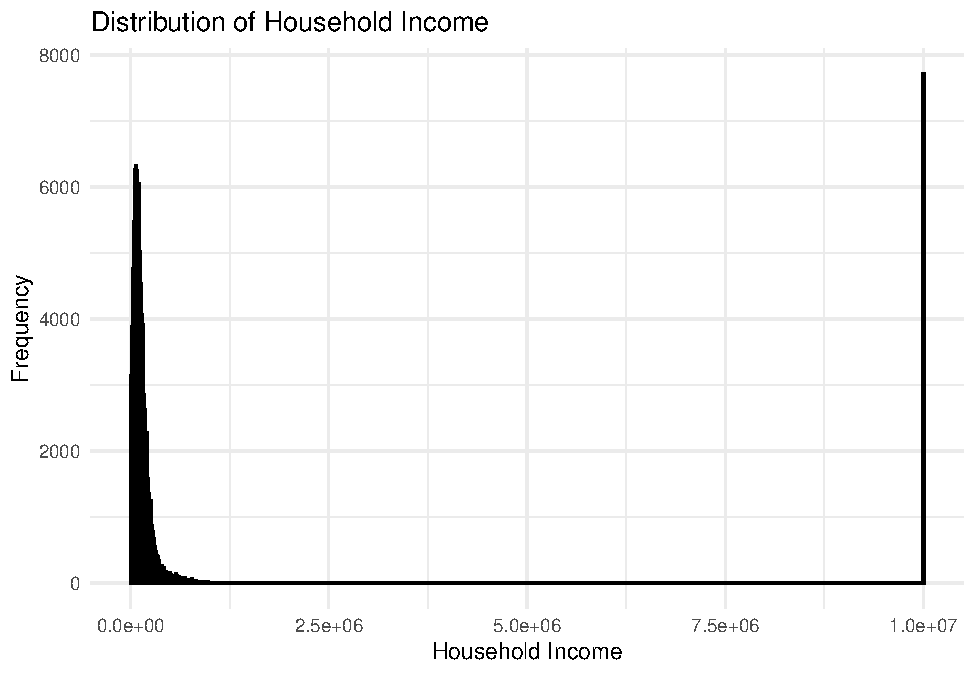
\includegraphics{Project_1_456_files/figure-latex/unnamed-chunk-6-1.pdf}

\subsection{Filtered Histogram}\label{filtered-histogram}

\subsubsection{AGE}\label{age-1}

We can see in the histogram for Age that there is a relatively normal
distribution with no skew and major outliers. so we have a fairly
balanced data set.

\begin{Shaded}
\begin{Highlighting}[]
\FunctionTok{ggplot}\NormalTok{(filtered\_data, }\FunctionTok{aes}\NormalTok{(}\AttributeTok{x =}\NormalTok{ AGE)) }\SpecialCharTok{+}
  \FunctionTok{geom\_histogram}\NormalTok{(}\AttributeTok{binwidth =} \DecValTok{5}\NormalTok{, }\AttributeTok{fill =} \StringTok{"blue"}\NormalTok{, }\AttributeTok{color =} \StringTok{"black"}\NormalTok{, }\AttributeTok{alpha =} \FloatTok{0.7}\NormalTok{) }\SpecialCharTok{+}
  \FunctionTok{labs}\NormalTok{(}\AttributeTok{title =} \StringTok{"Distribution of Age"}\NormalTok{, }\AttributeTok{x =} \StringTok{"Age"}\NormalTok{, }\AttributeTok{y =} \StringTok{"Frequency"}\NormalTok{) }\SpecialCharTok{+}
  \FunctionTok{theme\_minimal}\NormalTok{()}
\end{Highlighting}
\end{Shaded}

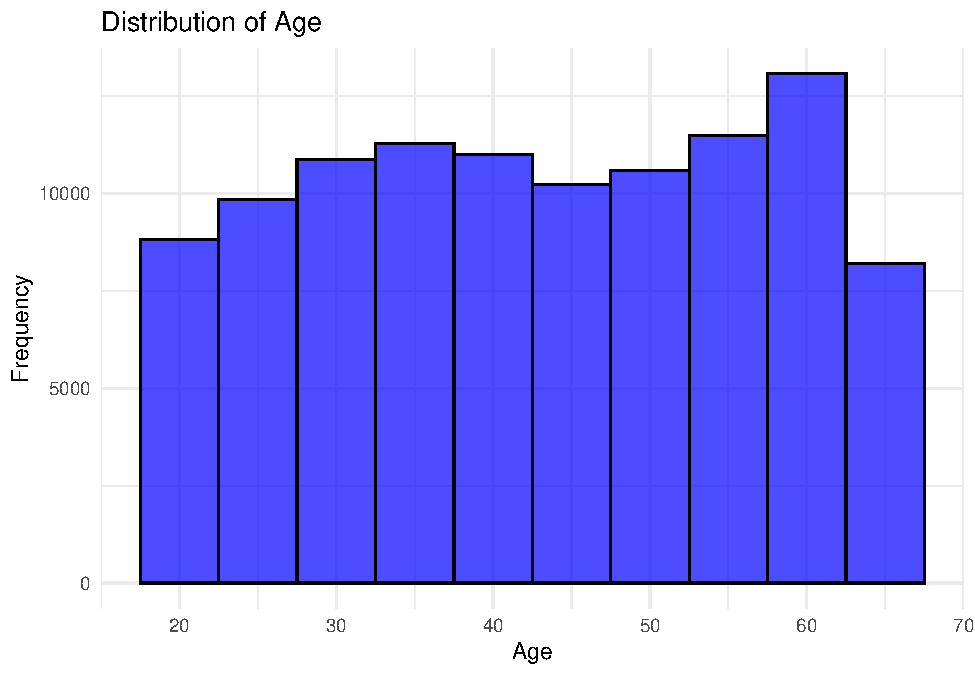
\includegraphics{Project_1_456_files/figure-latex/unnamed-chunk-7-1.pdf}

\subsubsection{Household Income}\label{household-income-1}

Although the data set still contains a right skew, The data is a lot
better of a fit for this instance. There are no extreme outliers and
actual as mentioned before that skew is bound to be prevalent over the
individual as most house holds in the data set earn a relatively modest
income

\begin{Shaded}
\begin{Highlighting}[]
\FunctionTok{ggplot}\NormalTok{(filtered\_data, }\FunctionTok{aes}\NormalTok{(}\AttributeTok{x =}\NormalTok{ HHINCOME)) }\SpecialCharTok{+}
  \FunctionTok{geom\_histogram}\NormalTok{(}\AttributeTok{binwidth =} \DecValTok{10000}\NormalTok{, }\AttributeTok{fill =} \StringTok{"green"}\NormalTok{, }\AttributeTok{color =} \StringTok{"black"}\NormalTok{, }\AttributeTok{alpha =} \FloatTok{0.7}\NormalTok{) }\SpecialCharTok{+}
  \FunctionTok{labs}\NormalTok{(}\AttributeTok{title =} \StringTok{"Distribution of Household Income"}\NormalTok{, }\AttributeTok{x =} \StringTok{"Household Income"}\NormalTok{, }\AttributeTok{y =} \StringTok{"Frequency"}\NormalTok{) }\SpecialCharTok{+}
  \FunctionTok{theme\_minimal}\NormalTok{()}
\end{Highlighting}
\end{Shaded}

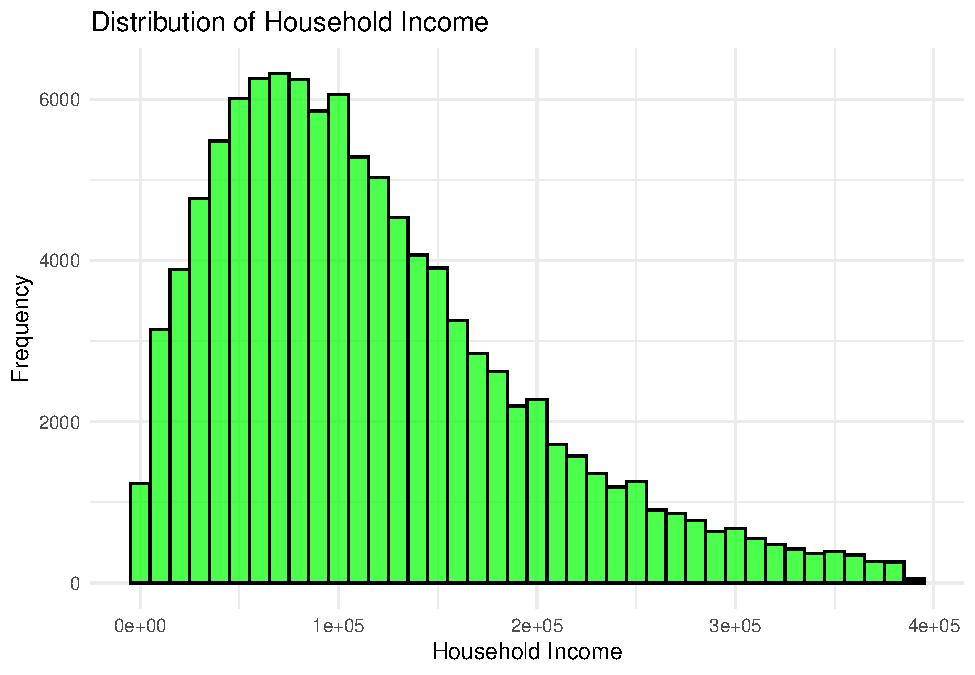
\includegraphics{Project_1_456_files/figure-latex/unnamed-chunk-8-1.pdf}

\subsection{Box Plots of original
data}\label{box-plots-of-original-data}

\subsubsection{AGE}\label{age-2}

\begin{Shaded}
\begin{Highlighting}[]
\FunctionTok{boxplot}\NormalTok{(data}\SpecialCharTok{$}\NormalTok{AGE, }\AttributeTok{main =} \StringTok{"Boxplot of Age"}\NormalTok{, }\AttributeTok{col =} \StringTok{"lightblue"}\NormalTok{, }\AttributeTok{ylab =} \StringTok{"Age"}\NormalTok{)}
\end{Highlighting}
\end{Shaded}

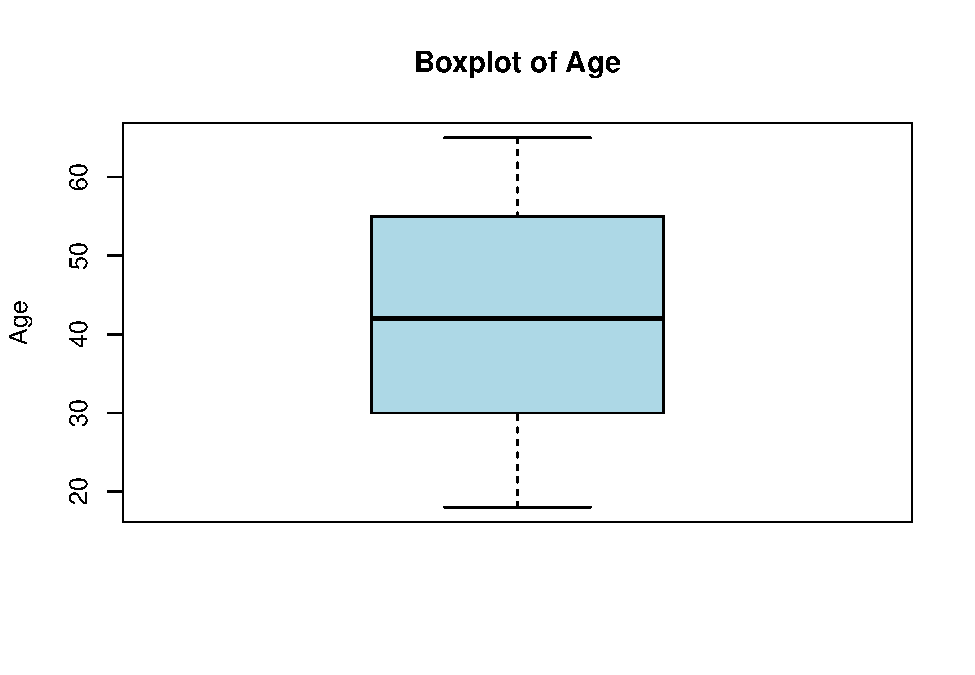
\includegraphics{Project_1_456_files/figure-latex/unnamed-chunk-9-1.pdf}

\subsubsection{Household Income}\label{household-income-2}

\begin{Shaded}
\begin{Highlighting}[]
\FunctionTok{boxplot}\NormalTok{(data}\SpecialCharTok{$}\NormalTok{HHINCOME, }\AttributeTok{main =} \StringTok{"Boxplot of Household Income"}\NormalTok{, }\AttributeTok{col =} \StringTok{"lightgreen"}\NormalTok{, }\AttributeTok{ylab =} \StringTok{"Household Income"}\NormalTok{, }\AttributeTok{ylim =} \FunctionTok{c}\NormalTok{(}\DecValTok{0}\NormalTok{, }\DecValTok{1000000}\NormalTok{))}
\end{Highlighting}
\end{Shaded}

\includegraphics{Project_1_456_files/figure-latex/unnamed-chunk-10-1.pdf}

\section{Analysis}\label{analysis}

\begin{Shaded}
\begin{Highlighting}[]
\CommentTok{\# modifying data into a training set and a testing set}
\FunctionTok{set.seed}\NormalTok{(}\DecValTok{1}\NormalTok{)}
\CommentTok{\# ask about a good metric for the split of the data}
\NormalTok{split }\OtherTok{\textless{}{-}} \FunctionTok{sample.split}\NormalTok{(filtered\_data}\SpecialCharTok{$}\NormalTok{HHINCOME, }\AttributeTok{SplitRatio =} \FloatTok{0.98}\NormalTok{)}
\NormalTok{train\_set }\OtherTok{\textless{}{-}} \FunctionTok{subset}\NormalTok{(filtered\_data, split }\SpecialCharTok{==} \ConstantTok{TRUE}\NormalTok{)}
\NormalTok{test\_set }\OtherTok{\textless{}{-}} \FunctionTok{subset}\NormalTok{(filtered\_data, split }\SpecialCharTok{==} \ConstantTok{FALSE}\NormalTok{)}

\CommentTok{\#sized of the sets}
\FunctionTok{cat}\NormalTok{(}\FunctionTok{paste}\NormalTok{(}\StringTok{"Size of the training set (rows):"}\NormalTok{, }\FunctionTok{nrow}\NormalTok{(train\_set), }\StringTok{"}\SpecialCharTok{\textbackslash{}n}\StringTok{"}\NormalTok{))}
\end{Highlighting}
\end{Shaded}

\begin{verbatim}
## Size of the training set (rows): 103723
\end{verbatim}

\begin{Shaded}
\begin{Highlighting}[]
\FunctionTok{cat}\NormalTok{(}\FunctionTok{paste}\NormalTok{(}\StringTok{"Size of the testing set (rows):"}\NormalTok{, }\FunctionTok{nrow}\NormalTok{(test\_set), }\StringTok{"}\SpecialCharTok{\textbackslash{}n}\StringTok{"}\NormalTok{))}
\end{Highlighting}
\end{Shaded}

\begin{verbatim}
## Size of the testing set (rows): 1660
\end{verbatim}

\begin{Shaded}
\begin{Highlighting}[]
\CommentTok{\#model from the training data}
\NormalTok{linear\_model }\OtherTok{\textless{}{-}} \FunctionTok{lm}\NormalTok{(HHINCOME }\SpecialCharTok{\textasciitilde{}}\NormalTok{ AGE, }\AttributeTok{data =}\NormalTok{ train\_set)}

\CommentTok{\# Prediceted values on the test set}
\NormalTok{test\_set}\SpecialCharTok{$}\NormalTok{predicted\_HHI }\OtherTok{\textless{}{-}} \FunctionTok{predict}\NormalTok{(linear\_model, }\AttributeTok{newdata =}\NormalTok{ test\_set)}

\CommentTok{\# calculate residuals for the test set}
\NormalTok{test\_set}\SpecialCharTok{$}\NormalTok{residuals }\OtherTok{\textless{}{-}}\NormalTok{ test\_set}\SpecialCharTok{$}\NormalTok{HHINCOME }\SpecialCharTok{{-}}\NormalTok{ test\_set}\SpecialCharTok{$}\NormalTok{predicted\_HHI}


\CommentTok{\# Display equation information for the simple linear regression}
\NormalTok{linear\_model}
\end{Highlighting}
\end{Shaded}

\begin{verbatim}
## 
## Call:
## lm(formula = HHINCOME ~ AGE, data = train_set)
## 
## Coefficients:
## (Intercept)          AGE  
##   115580.53        33.32
\end{verbatim}

For the data set, we implemented 98\% (103,723 points) of filtered data
options goes towards training our model. The large percentage was used
due to the Extreme scale of data we are implementing. The Testing set
implemented 2\% (1,660 points) of the data and we implemented for the
testing and assessment of our regression algorithm.

Thus Through our training data we get the The following regression model
\[
HHINCOME = 115580.53 + 33.32 \times AGE
\] Which we can streamline down into the following linear regression
problem

\[ 
y = 115580.53 + 33.32 x_1
\]

\subsection{Implementing the Plots}\label{implementing-the-plots}

\subsubsection{Linear Regression with Training
Data}\label{linear-regression-with-training-data}

\begin{Shaded}
\begin{Highlighting}[]
\FunctionTok{plot}\NormalTok{(train\_set}\SpecialCharTok{$}\NormalTok{AGE, train\_set}\SpecialCharTok{$}\NormalTok{HHINCOME, }\AttributeTok{main=}\StringTok{"HHINCOME vs AGE"}\NormalTok{, }\AttributeTok{xlab=}\StringTok{"Age"}\NormalTok{, }\AttributeTok{ylab=}\StringTok{"Household Income"}\NormalTok{)}

\CommentTok{\# Fit the linear regression model}
\NormalTok{model }\OtherTok{\textless{}{-}} \FunctionTok{lm}\NormalTok{(HHINCOME }\SpecialCharTok{\textasciitilde{}}\NormalTok{ AGE, }\AttributeTok{data =}\NormalTok{ train\_set)}

\CommentTok{\# Add the regression line to the plot}
\FunctionTok{abline}\NormalTok{(model, }\AttributeTok{col=}\StringTok{"red"}\NormalTok{)}
\end{Highlighting}
\end{Shaded}

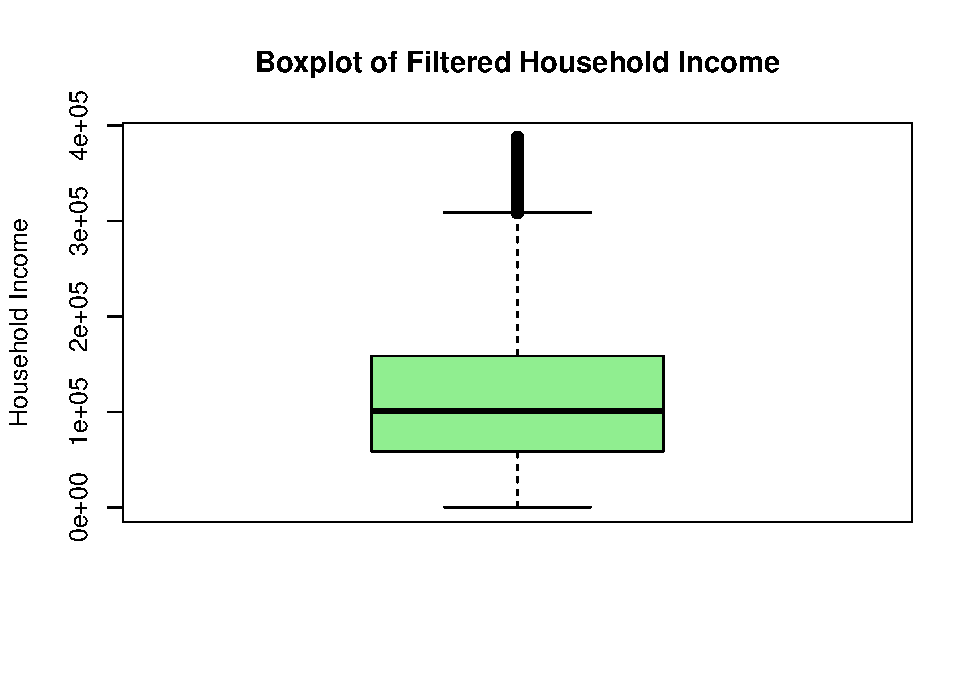
\includegraphics{Project_1_456_files/figure-latex/unnamed-chunk-12-1.pdf}

We can see with the diaganol with the original training set is that it
is almost impossible to deter how good of a fit the line is. There are
simply to many points in the model to decipher a strong linear
regression.

\subsubsection{Linear Regression with Testing
Data}\label{linear-regression-with-testing-data}

This plot is also referenced in the next session for further assessment.

\begin{Shaded}
\begin{Highlighting}[]
\FunctionTok{plot}\NormalTok{(test\_set}\SpecialCharTok{$}\NormalTok{AGE, test\_set}\SpecialCharTok{$}\NormalTok{HHINCOME, }\AttributeTok{main=}\StringTok{"HHINCOME vs AGE"}\NormalTok{, }\AttributeTok{xlab=}\StringTok{"Age"}\NormalTok{, }\AttributeTok{ylab=}\StringTok{"Household Income"}\NormalTok{)}

\CommentTok{\# Fit the linear regression model}
\NormalTok{model }\OtherTok{\textless{}{-}} \FunctionTok{lm}\NormalTok{(HHINCOME }\SpecialCharTok{\textasciitilde{}}\NormalTok{ AGE, }\AttributeTok{data =}\NormalTok{ train\_set)}

\CommentTok{\# Add the regression line to the plot}
\FunctionTok{abline}\NormalTok{(model, }\AttributeTok{col=}\StringTok{"red"}\NormalTok{)}
\end{Highlighting}
\end{Shaded}

\includegraphics{Project_1_456_files/figure-latex/unnamed-chunk-13-1.pdf}

From our model we can see that the linear regression line is an
extremely poor fit and in fact actually resembles the set up of the
residual vs fitted value graphs.

This output further suggest that a linear regression model is not
appropriate for the data, as the residuals show the lower cluster
patterns, and the separate data points for the testing points appear to
fail to encompass the model with any sort of trends.

\subsubsection{Summary of the Simple Linear Regression
Model}\label{summary-of-the-simple-linear-regression-model}

\begin{Shaded}
\begin{Highlighting}[]
\FunctionTok{summary}\NormalTok{(linear\_model)}
\end{Highlighting}
\end{Shaded}

\begin{verbatim}
## 
## Call:
## lm(formula = HHINCOME ~ AGE, data = train_set)
## 
## Residuals:
##     Min      1Q  Median      3Q     Max 
## -117716  -58313  -16213   41987  271020 
## 
## Coefficients:
##              Estimate Std. Error t value Pr(>|t|)    
## (Intercept) 115580.53     787.18 146.829   <2e-16 ***
## AGE             33.32      17.47   1.907   0.0565 .  
## ---
## Signif. codes:  0 '***' 0.001 '**' 0.01 '*' 0.05 '.' 0.1 ' ' 1
## 
## Residual standard error: 78150 on 103721 degrees of freedom
## Multiple R-squared:  3.506e-05,  Adjusted R-squared:  2.542e-05 
## F-statistic: 3.636 on 1 and 103721 DF,  p-value: 0.05653
\end{verbatim}

From the Residual ranges we can see that the linear model has some very
large error when it comes to underestimating and overestimating a US
citizens house hold income. Our coefficient for the Age of a person is
33.32 meaning that the model predicts that for every additional year of
age, household income increases by 33.32 dollars on average. this is an
extremely small change which can only mean the age alone is not a very
strong depiction of income in our linear model.

With this Our predicted linear equation is

\section{Model Evaluation and
Prediction}\label{model-evaluation-and-prediction}

\subsubsection{Model Assessment}\label{model-assessment}

\begin{Shaded}
\begin{Highlighting}[]
\FunctionTok{ggplot}\NormalTok{(test\_set, }\FunctionTok{aes}\NormalTok{(}\AttributeTok{x =}\NormalTok{ predicted\_HHI, }\AttributeTok{y =}\NormalTok{ residuals)) }\SpecialCharTok{+}
  \FunctionTok{geom\_point}\NormalTok{(}\AttributeTok{alpha =} \FloatTok{0.5}\NormalTok{, }\AttributeTok{color =} \StringTok{\textquotesingle{}black\textquotesingle{}}\NormalTok{) }\SpecialCharTok{+}
  \FunctionTok{geom\_hline}\NormalTok{(}\AttributeTok{yintercept =} \DecValTok{0}\NormalTok{, }\AttributeTok{linetype =} \StringTok{"dashed"}\NormalTok{, }\AttributeTok{color =} \StringTok{"red"}\NormalTok{) }\SpecialCharTok{+}
  \FunctionTok{labs}\NormalTok{(}\AttributeTok{title =} \StringTok{"Residuals vs. Fitted Values"}\NormalTok{,}
       \AttributeTok{x =} \StringTok{"Fitted Values"}\NormalTok{,}
       \AttributeTok{y =} \StringTok{"Residuals"}\NormalTok{) }\SpecialCharTok{+}
  \FunctionTok{theme\_minimal}\NormalTok{()}
\end{Highlighting}
\end{Shaded}

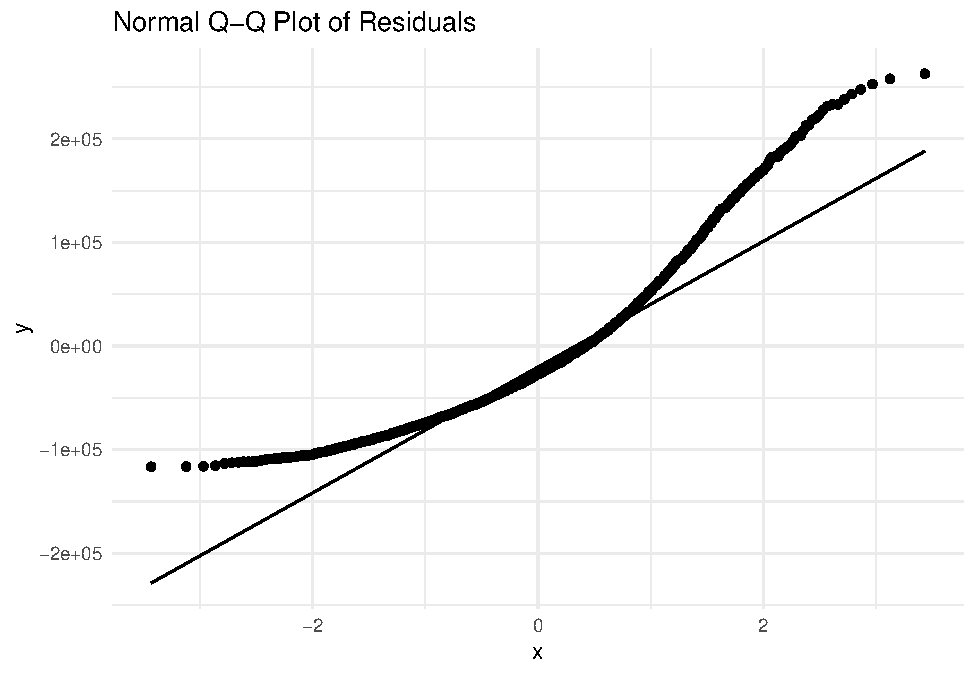
\includegraphics{Project_1_456_files/figure-latex/unnamed-chunk-15-1.pdf}

Observe this Residuals vs.~Fitted Values plot.

The first thing we need to consider is whether the residuals are
randomly distributed around the zero line. Here there are clearly more
points below the line than above. This means that our model is likely to
overestimate household income and isn't doing a good job.

The second consideration is the pattern of the residuals. The fact that
the residuals appear with in a higher density towards the bottom points
towards our model not being a good fit.

The third consideration is the spread of the residuals across the range
of the fitted values. This appears to be good since the graph is
horizontally consistent.

The final consideration is if there are any outliers. We already
filtered the data for outliers so this is not a problem here.

\begin{Shaded}
\begin{Highlighting}[]
\FunctionTok{ggplot}\NormalTok{(test\_set, }\FunctionTok{aes}\NormalTok{(}\AttributeTok{sample =}\NormalTok{ residuals)) }\SpecialCharTok{+}
  \FunctionTok{stat\_qq}\NormalTok{() }\SpecialCharTok{+}
  \FunctionTok{stat\_qq\_line}\NormalTok{() }\SpecialCharTok{+}
  \FunctionTok{labs}\NormalTok{(}\AttributeTok{title =} \StringTok{"Normal Q{-}Q Plot of Residuals"}\NormalTok{) }\SpecialCharTok{+}
  \FunctionTok{theme\_minimal}\NormalTok{()}
\end{Highlighting}
\end{Shaded}

\includegraphics{Project_1_456_files/figure-latex/unnamed-chunk-16-1.pdf}

The Q-Q plot shown here is meant to help us see how normal our data is.
If the points fall close to the diagonal line, it is normally
distributed. If the data falls far from the line, it is not normally
distributed. In this case, the plot shows significant deviations from
the line, especially in the tails, indicating that the residuals are not
normally distributed. This non-normality suggests potential issues with
the model, such as missing important predictor variables, the presence
of outliers, or non-linearity in the data. Consequently, the assumption
of normally distributed residuals is violated, which can impact the
reliability of certain statistical tests and confidence intervals.

\textbf{Goodness-of-Fit:} - \textbf{R-squared Value:} Indicates the
proportion of variance in the dependent variable explained by the model.
- \textbf{Adjusted R-squared Value:} Adjusted for the number of
predictors in the model.

\begin{Shaded}
\begin{Highlighting}[]
\NormalTok{adjusted\_r\_squared }\OtherTok{\textless{}{-}} \FunctionTok{summary}\NormalTok{(linear\_model)}\SpecialCharTok{$}\NormalTok{r.squared}
\NormalTok{adjusted\_r\_squared}
\end{Highlighting}
\end{Shaded}

\begin{verbatim}
## [1] 3.505868e-05
\end{verbatim}

From our extremely low R-sqaured Value, we can conclude that AGE in this
instance has no Variability in household income. In other words, Age and
house hold income's relationship is extremely week

\begin{Shaded}
\begin{Highlighting}[]
\NormalTok{adjusted\_r\_squared }\OtherTok{\textless{}{-}} \FunctionTok{summary}\NormalTok{(linear\_model)}\SpecialCharTok{$}\NormalTok{adj.r.squared}
\NormalTok{adjusted\_r\_squared}
\end{Highlighting}
\end{Shaded}

\begin{verbatim}
## [1] 2.541777e-05
\end{verbatim}

While using the adjusted R-squared model to prevent overfitting of the
data, we can see that the data is relatively close to our initial
R-sqaured. Due to the fact the simple linear regression model uses only
one independent variable, this would lead to a simaler range in
output.this reinforces our interpretation of the age variable not being
a significant influence on the household income.

\subsubsection{Model Accuracy}\label{model-accuracy}

\textbf{Error Metrics:} - \textbf{Mean Squared Error (MSE):} Measures
the average squared difference between actual and predicted values.

\begin{Shaded}
\begin{Highlighting}[]
\NormalTok{r }\OtherTok{\textless{}{-}} \FunctionTok{as.vector}\NormalTok{(test\_set}\SpecialCharTok{$}\NormalTok{residuals)}
\NormalTok{mse }\OtherTok{\textless{}{-}} \FunctionTok{mean}\NormalTok{(r}\SpecialCharTok{\^{}}\DecValTok{2}\NormalTok{)}
\NormalTok{mse}
\end{Highlighting}
\end{Shaded}

\begin{verbatim}
## [1] 4886139175
\end{verbatim}

The Mean Squared Error displays an extremely high number.this means
there is a large difference between the predicted output of a actual and
predicted output of someone's income.The output further enforces the
inadequacy of the linear regression model.

\subsubsection{Prediction}\label{prediction}

\textbf{Prediction vs.~Actual Plot:}

\begin{Shaded}
\begin{Highlighting}[]
\FunctionTok{plot}\NormalTok{(test\_set}\SpecialCharTok{$}\NormalTok{AGE, test\_set}\SpecialCharTok{$}\NormalTok{HHINCOME, }\AttributeTok{main=}\StringTok{"Prediction vs Actual"}\NormalTok{, }
     \AttributeTok{xlab=}\StringTok{"Age"}\NormalTok{, }\AttributeTok{ylab=}\StringTok{"Household Income"}\NormalTok{, }\AttributeTok{pch=}\DecValTok{16}\NormalTok{, }\AttributeTok{col=}\StringTok{"blue"}\NormalTok{)}

\CommentTok{\# add linear regression model}
\NormalTok{model }\OtherTok{\textless{}{-}} \FunctionTok{lm}\NormalTok{(HHINCOME }\SpecialCharTok{\textasciitilde{}}\NormalTok{ AGE, }\AttributeTok{data =}\NormalTok{ train\_set)}
\FunctionTok{abline}\NormalTok{(model, }\AttributeTok{col=}\StringTok{"red"}\NormalTok{, }\AttributeTok{lwd=}\DecValTok{3}\NormalTok{)}
\end{Highlighting}
\end{Shaded}

\includegraphics{Project_1_456_files/figure-latex/unnamed-chunk-20-1.pdf}

\section{Conclusion and Summary}\label{conclusion-and-summary}

Our simple linear regression model for the Comparison of United States
Household income and resident age from the IPUM USA data. WE were able
to derive a linear regression model from a training set of 103,723
points to derive the Equation below. \[
HHINCOME = 115580.53 + 33.32 \times AGE
\] This equation indicates that the increase in a person's age in the
discrete model had an almost negligible effect on the amount they could
contribute to their household income. This suggests that, overall, there
is minimal income growth on a yearly basis for individuals. Our
R-squared value of 3.51e-05 and adjusted R-squared value of 2.54e-05
show that this model had almost no correlation at all with the testing
set. This was also reflected in the graph of the derived regression
equation and the actual predicted values, which followed no discernible
trends and resembled a residual plot more than an actual regression
model. Our mean squared error, which resulted in approximately 4.89
billion, highlights the presence of extreme outliers and significant
differences between our predicted and actual values. Through our
residual fitted values we can further visualize that the regression
model very rarely ever comes close to predicting the actual value of a
lot of our points. When we start to map out the Q-Q plot we also notice
that there is a week linear correlation on the diagonal and that the
data set is has alot of outliers present on the lower and the upper
portions of our model with these heavier tails.

A positive outcome from this model is that it establishes a baseline
comparison for future improvements in the modeling process. This model
allows us to explore different mathematical modeling approaches and
refine our data processing methods for a more optimal setup.
Additionally, the residual-based calculations emphasized the need to
reconsider our original data selection, suggesting that household income
may have a much stronger correlation with other independent variables
present in the data set.

The model also has drawbacks. The large data set made it difficult to
perform an efficient analysis without long computing times, requiring us
to reduce the data size and introduce a seed. Although this was done
through a randomized selection approach, it may have affected the
selection of appropriate data. Furthermore, the data set exhibited
potential bias, as a significant portion of those surveyed came from
modest to lower-income households, leading to a skewed data set.

Regardless of how we interpret our findings, it is evident that moving
to another modeling approach is necessary to better understand the
factors affecting household income in the United States. Given the
limitations of simple linear regression, a multivariate linear
regression model would be a more optimal approach, allowing us to
incorporate additional variables to enable predictive accuracy.
Additionally, having access to more dynamic and optimal testing methods,
including Cross Validation selection, F-tests, Residual Error
Independence and many more testing methods , will enable us to build a
more robust and efficient model. By refining our techniques, we can
develop a stronger predictive model that better represents the
complexities of household income distribution.

\section{Reference}\label{reference}

Sources cited:

\#1 Steven Ruggles, Sarah Flood, Matthew Sobek, Daniel Backman, Annie
Chen, Grace Cooper, Stephanie Richards, Renae Rodgers, and Megan
Schouweiler. IPUMS USA: Version 15.0 {[}dataset{]} Minneapolis, MN:
IPUMS, 2024. \url{https://doi.org/10.18128/D010.V15.0}

\#2 Benabou, Roland, and Efe A. Ok. ``Social Mobility and the Demand for
Redistribution: The Poum Hypothesis.'' The Quarterly Journal of
Economics 116, no. 2 (2001): 447--87.
\url{http://www.jstor.org/stable/2696470}.

\#3 Solon, Gary. ``Intergenerational Income Mobility in the United
States.'' The American Economic Review 82, no. 3 (1992): 393--408.
\url{http://www.jstor.org/stable/2117312}.

\end{document}
